% McKinsey-Style Report: The Agent Infrastructure Stack
% Compile with: tectonic mckinsey_report.tex
\documentclass[11pt,a4paper]{article}

% ─── Core packages ───
\usepackage[a4paper, top=25mm, bottom=25mm, left=25mm, right=25mm]{geometry}
\usepackage{graphicx}
\usepackage{xcolor}
\usepackage{tikz}
\usetikzlibrary{calc,positioning,shapes.geometric,arrows.meta,backgrounds,fit,decorations.markings,patterns}
\usepackage{fontspec}
\usepackage{titlesec}
\usepackage{enumitem}
\usepackage{tabularx}
\usepackage{booktabs}
\usepackage{multicol}
\usepackage{fancyhdr}
\usepackage{hyperref}
\usepackage{parskip}
\usepackage{ragged2e}
\usepackage{microtype}
\usepackage{changepage}
\usepackage{wrapfig}
\usepackage{colortbl}
\usepackage{array}
\usepackage{calc}
\usepackage{eso-pic}
\usepackage{afterpage}
\usepackage{pgfplots}
\pgfplotsset{compat=1.18}

% ─── Fonts ───
\setmainfont{Helvetica Neue}[
  UprightFont = *,
  BoldFont = * Bold,
  ItalicFont = * Italic,
  BoldItalicFont = * Bold Italic,
]
\setsansfont{Helvetica Neue}[
  UprightFont = *,
  BoldFont = * Bold,
  ItalicFont = * Italic,
]

% ─── Color Palette (McKinsey-inspired) ───
\definecolor{navy}{HTML}{0A1628}
\definecolor{darkblue}{HTML}{1A2744}
\definecolor{primary}{HTML}{2563EB}
\definecolor{accent}{HTML}{3B82F6}
\definecolor{lightblue}{HTML}{DBEAFE}
\definecolor{lightbluebg}{HTML}{EFF6FF}
\definecolor{warmgray}{HTML}{F8F7F4}
\definecolor{textmain}{HTML}{1E293B}
\definecolor{textsub}{HTML}{64748B}
\definecolor{success}{HTML}{059669}
\definecolor{warning}{HTML}{D97706}
\definecolor{danger}{HTML}{DC2626}
\definecolor{chartblue}{HTML}{2563EB}
\definecolor{chartteal}{HTML}{0D9488}
\definecolor{chartpurple}{HTML}{7C3AED}
\definecolor{chartamber}{HTML}{D97706}
\definecolor{chartrose}{HTML}{E11D48}
\definecolor{tablegray}{HTML}{F1F5F9}
\definecolor{tableborder}{HTML}{E2E8F0}

% ─── Hyperref ───
\hypersetup{
  colorlinks=true,
  linkcolor=primary,
  urlcolor=primary,
  pdfauthor={Vedang Ratan Vatsa},
  pdftitle={The Agent Infrastructure Stack},
}

% ─── Page style ───
\pagestyle{fancy}
\fancyhf{}
\renewcommand{\headrulewidth}{0pt}
\fancyfoot[L]{\footnotesize\color{textsub}The Agent Infrastructure Stack}
\fancyfoot[R]{\footnotesize\color{textsub}\thepage}

% ─── Section formatting ───
\titleformat{\section}
  {\fontsize{22}{26}\selectfont\bfseries\color{navy}}
  {}
  {0pt}
  {}
\titlespacing*{\section}{0pt}{30pt}{12pt}

\titleformat{\subsection}
  {\fontsize{15}{19}\selectfont\bfseries\color{darkblue}}
  {}
  {0pt}
  {}
\titlespacing*{\subsection}{0pt}{22pt}{8pt}

\titleformat{\subsubsection}
  {\fontsize{12}{15}\selectfont\bfseries\color{primary}}
  {}
  {0pt}
  {}
\titlespacing*{\subsubsection}{0pt}{16pt}{6pt}

% ─── Custom commands ───

% Stat callout box (big number + label)
\newcommand{\statbox}[3]{% width, number, label
  \begin{tikzpicture}
    \node[
      rectangle,
      rounded corners=6pt,
      fill=lightbluebg,
      draw=lightblue,
      line width=0.5pt,
      minimum width=#1,
      minimum height=22mm,
      inner sep=6pt,
    ] {
      \begin{minipage}{#1-14pt}
      \centering
      {\fontsize{28}{32}\selectfont\bfseries\color{primary}#2}\\[3pt]
      {\fontsize{9}{11}\selectfont\color{textsub}#3}
      \end{minipage}
    };
  \end{tikzpicture}%
}

% Pull quote
\newcommand{\pullquote}[1]{%
  \begin{center}
  \begin{tikzpicture}
    \node[
      rectangle,
      rounded corners=4pt,
      fill=warmgray,
      minimum width=0.88\textwidth,
      inner sep=14pt,
      align=center,
      text width=0.82\textwidth,
    ] {
      \begin{minipage}{0.82\textwidth}
      \begin{center}
      {\fontsize{13}{17}\selectfont\itshape\color{darkblue}#1}
      \end{center}
      \end{minipage}
    };
  \end{tikzpicture}
  \end{center}
}

% Key insight box
\newcommand{\insightbox}[2]{% title, content
  \begin{tikzpicture}
    \node[
      rectangle,
      rounded corners=6pt,
      fill=navy,
      minimum width=\textwidth,
      inner sep=14pt,
      text width=\textwidth-32pt,
    ] {
      {\fontsize{11}{13}\selectfont\bfseries\color{accent}#1}\\[6pt]
      {\fontsize{10}{14}\selectfont\color{white}#2}
    };
  \end{tikzpicture}
}

% Section divider
\newcommand{\sectiondivider}{%
  \vspace{8pt}
  \noindent
\begin{tikzpicture}
    \fill[primary] (0,0) rectangle (\textwidth, 2pt);
  \end{tikzpicture}
  \vspace{6pt}
}

% Full-width colored banner for section headers
\newcommand{\sectionbanner}[2]{% section number, title
  \vspace{15pt}
  \noindent\begin{tikzpicture}
    \node[
      rectangle,
      rounded corners=4pt,
      fill=navy,
      minimum width=\textwidth,
      minimum height=16mm,
      inner sep=10pt,
      anchor=west,
    ] at (0,0) {
      \begin{minipage}{\textwidth-24pt}
        {\fontsize{10}{12}\selectfont\color{accent}\bfseries SECTION #1}\\[2pt]
        {\fontsize{18}{22}\selectfont\bfseries\color{white}#2}
      \end{minipage}
    };
  \end{tikzpicture}
  \vspace{10pt}
}


% ════════════════════════════════════════════════════════════
% DOCUMENT BEGINS
% ════════════════════════════════════════════════════════════

\begin{document}
\color{textmain}

% ─── COVER PAGE ───
\thispagestyle{empty}
\newgeometry{margin=0pt}
\begin{tikzpicture}[remember picture, overlay]
  % Background
  \fill[navy] (current page.south west) rectangle (current page.north east);
  
  % Cover image (positioned in upper-right area)
  \node[anchor=center, opacity=0.35] at ([yshift=-4cm]current page.center) {
    \includegraphics[width=\paperwidth]{report_cover.png}
  };
  
  % Gradient overlay from bottom
  \fill[navy, opacity=0.7] (current page.south west) rectangle ([yshift=12cm]current page.south east);
  
  % Accent line
  \fill[primary] ([xshift=40mm, yshift=145mm]current page.south west) rectangle ([xshift=100mm, yshift=148mm]current page.south west);
  
  % Report type label
  \node[anchor=west, text=accent] at ([xshift=40mm, yshift=158mm]current page.south west) {
    {\fontsize{11}{13}\selectfont\bfseries\addfontfeatures{LetterSpace=8}RESEARCH REPORT \hspace{4pt}|\hspace{4pt} MAY 2026}
  };
  
  % Main title
  \node[anchor=west, text width=130mm] at ([xshift=40mm, yshift=118mm]current page.south west) {
    {\fontsize{38}{42}\selectfont\bfseries\color{white}The Agent\\Infrastructure\\Stack}
  };
  
  % Subtitle
  \node[anchor=west, text width=120mm] at ([xshift=40mm, yshift=72mm]current page.south west) {
    {\fontsize{14}{19}\selectfont\color{white!75!navy}Taxonomy, Capital Flows, and Consolidation\\in the \$13B Developer Toolchain for\\Autonomous AI Systems}
  };
  
  % Author
  \node[anchor=west] at ([xshift=40mm, yshift=42mm]current page.south west) {
    {\fontsize{11}{13}\selectfont\color{white!60!navy}Vedang Ratan Vatsa}
  };
  \node[anchor=west] at ([xshift=40mm, yshift=35mm]current page.south west) {
    {\fontsize{9}{11}\selectfont\color{white!40!navy}vedangvats@gmail.com}
  };
  
  % Bottom accent bar
  \fill[primary] ([yshift=18mm]current page.south west) rectangle ([yshift=18.5mm]current page.south east);
\end{tikzpicture}
\restoregeometry
\clearpage


% ─── EXECUTIVE SUMMARY PAGE ───
\thispagestyle{empty}

\vspace*{-5mm}

\noindent
\begin{tikzpicture}
  \fill[primary] (0,0) rectangle (\textwidth, 1.5pt);
\end{tikzpicture}

\vspace{4mm}

{\fontsize{10}{12}\selectfont\bfseries\color{primary}\addfontfeatures{LetterSpace=6}EXECUTIVE SUMMARY}

\vspace{6mm}

{\fontsize{22}{26}\selectfont\bfseries\color{navy}The developer toolchain for AI agents has\\split into eight infrastructure layers,\\attracting \$13B in 24 months.}

\vspace{10mm}

% Key stats row
\noindent\hfill
\statbox{45mm}{\$13B}{Total Disclosed Funding}
\hfill
\statbox{45mm}{50+}{Companies Analyzed}
\hfill
\statbox{45mm}{85\%}{Capital in Top 10 Deals}
\hfill\null

\vspace{10mm}

\noindent\begin{tikzpicture}
  \fill[tableborder] (0,0) rectangle (\textwidth, 0.5pt);
\end{tikzpicture}

\vspace{6mm}

\begin{multicols}{2}
\setlength{\parskip}{6pt}

{\fontsize{10}{14}\selectfont

\textbf{\color{navy}The opportunity.} Between 2024 and 2026, the developer toolchain for building AI agents split into eight specialized infrastructure layers. Each layer attracted dedicated venture-backed companies and approximately \$13 billion in combined disclosed funding.

\textbf{\color{navy}Capital concentration is extreme.} The top 3 deals (Cognition, Groq, Sierra) account for roughly 46\% of total disclosed capital. Compute and agent products together take 85\% of total funding, leaving six middleware layers to split \$1.6B.

\textbf{\color{navy}Consolidation has begun.} Security and observability companies are being acquired by platform incumbents (Cisco, Check Point, ClickHouse). Five of eight acquisitions in this dataset occurred in these two layers.

\textbf{\color{navy}The structure is transitional.} Enterprise surveys show 60\% of organizations plan agent deployment within two years, but only 17\% have deployed. This gap creates demand that infrastructure companies fill---but also existential risk if agents fail to deliver expected value.

}
\end{multicols}

\vspace{6mm}

\insightbox{KEY FINDING}{The eight-layer structure will likely consolidate to approximately five within three years. Security and observability are headed toward platform absorption. Memory will commoditize into general-purpose databases. Compute, perception, and orchestration appear positioned to remain independent.}

\clearpage


% ─── TABLE OF CONTENTS ───
\thispagestyle{empty}

\vspace*{-5mm}

\noindent
\begin{tikzpicture}
  \fill[primary] (0,0) rectangle (\textwidth, 1.5pt);
\end{tikzpicture}

\vspace{4mm}

{\fontsize{10}{12}\selectfont\bfseries\color{primary}\addfontfeatures{LetterSpace=6}CONTENTS}

\vspace{8mm}

\renewcommand{\arraystretch}{2.0}
\noindent\begin{tabularx}{\textwidth}{@{} >{\fontsize{28}{32}\selectfont\color{primary!30}\bfseries}r @{\hspace{10pt}} >{\raggedright\arraybackslash}X @{}}
01 & {\fontsize{14}{17}\selectfont\bfseries\color{navy}The Eight-Layer Taxonomy}\newline{\fontsize{9.5}{12}\selectfont\color{textsub}How the agent infrastructure stack is organized and why} \\[2pt]
\arrayrulecolor{tableborder}\hline
02 & {\fontsize{14}{17}\selectfont\bfseries\color{navy}Market Analysis}\newline{\fontsize{9.5}{12}\selectfont\color{textsub}Capital concentration, revenue multiples, and commoditization signals} \\[2pt]
\hline
03 & {\fontsize{14}{17}\selectfont\bfseries\color{navy}Architectural Trends}\newline{\fontsize{9.5}{12}\selectfont\color{textsub}Six shifts from pre-agent to agent-first infrastructure} \\[2pt]
\hline
04 & {\fontsize{14}{17}\selectfont\bfseries\color{navy}Consolidation Dynamics}\newline{\fontsize{9.5}{12}\selectfont\color{textsub}Who acquires, what stays independent, and why} \\[2pt]
\hline
05 & {\fontsize{14}{17}\selectfont\bfseries\color{navy}Platform Convergence}\newline{\fontsize{9.5}{12}\selectfont\color{textsub}Marketplace bundling and the AWS parallel} \\[2pt]
\hline
06 & {\fontsize{14}{17}\selectfont\bfseries\color{navy}Capital Allocation}\newline{\fontsize{9.5}{12}\selectfont\color{textsub}Funding velocity, investor thesis, and geographic concentration} \\[2pt]
\hline
07 & {\fontsize{14}{17}\selectfont\bfseries\color{navy}Open Questions and Outlook}\newline{\fontsize{9.5}{12}\selectfont\color{textsub}Risks, limitations, and what comes next} \\
\end{tabularx}

\clearpage


% ═══════════════════════════════════
% SECTION 1: THE EIGHT-LAYER TAXONOMY
% ═══════════════════════════════════
\sectionbanner{01}{The Eight-Layer Taxonomy}

{\fontsize{10.5}{15}\selectfont

The taxonomy groups companies into eight layers based on three separation criteria: independent scaling, distinct buyer persona, and separable billing. Each layer can grow its user base without requiring proportional growth in another layer.

}

\vspace{8mm}

% ─── INFOGRAPHIC: The Eight Layers ───
\noindent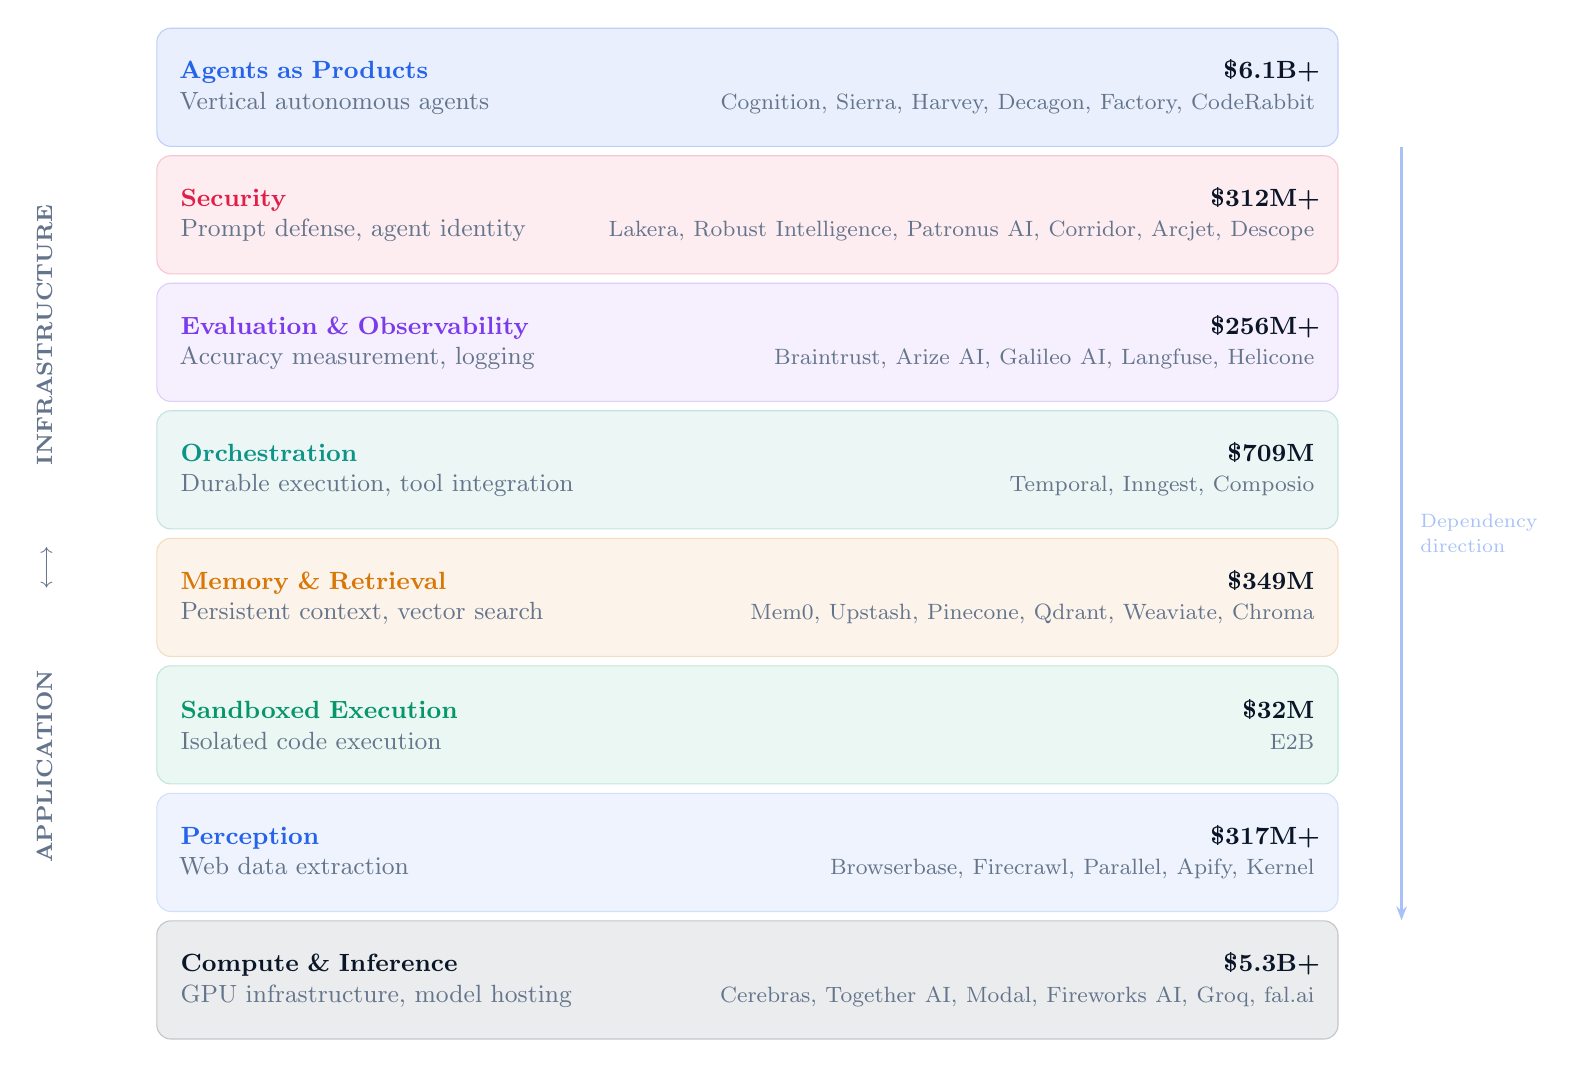
\begin{tikzpicture}[
  layerbox/.style={
    rectangle, rounded corners=5pt, 
    minimum width=150mm, minimum height=15mm,
    inner sep=6pt, text width=144mm,
    font=\fontsize{9.5}{12}\selectfont,
  },
]

% Layer 1 - Agents as Products
\node[layerbox, fill=primary!10, draw=primary!30] (l1) at (0, 0) {
  \textbf{\color{primary}Agents as Products} \hfill {\bfseries\color{navy}\$6.1B+}\\[-1pt]
  {\color{textsub}Vertical autonomous agents} \hfill {\color{textsub}\footnotesize Cognition, Sierra, Harvey, Decagon, Factory, CodeRabbit}
};

% Layer 2 - Security
\node[layerbox, fill=chartrose!8, draw=chartrose!25, below=3pt of l1] (l2) {
  \textbf{\color{chartrose}Security} \hfill {\bfseries\color{navy}\$312M+}\\[-1pt]
  {\color{textsub}Prompt defense, agent identity} \hfill {\color{textsub}\footnotesize Lakera, Robust Intelligence, Patronus AI, Corridor, Arcjet, Descope}
};

% Layer 3 - Eval & Observability
\node[layerbox, fill=chartpurple!8, draw=chartpurple!25, below=3pt of l2] (l3) {
  \textbf{\color{chartpurple}Evaluation \& Observability} \hfill {\bfseries\color{navy}\$256M+}\\[-1pt]
  {\color{textsub}Accuracy measurement, logging} \hfill {\color{textsub}\footnotesize Braintrust, Arize AI, Galileo AI, Langfuse, Helicone}
};

% Layer 4 - Orchestration
\node[layerbox, fill=chartteal!8, draw=chartteal!25, below=3pt of l3] (l4) {
  \textbf{\color{chartteal}Orchestration} \hfill {\bfseries\color{navy}\$709M}\\[-1pt]
  {\color{textsub}Durable execution, tool integration} \hfill {\color{textsub}\footnotesize Temporal, Inngest, Composio}
};

% Layer 5 - Memory & Retrieval
\node[layerbox, fill=chartamber!8, draw=chartamber!25, below=3pt of l4] (l5) {
  \textbf{\color{chartamber}Memory \& Retrieval} \hfill {\bfseries\color{navy}\$349M}\\[-1pt]
  {\color{textsub}Persistent context, vector search} \hfill {\color{textsub}\footnotesize Mem0, Upstash, Pinecone, Qdrant, Weaviate, Chroma}
};

% Layer 6 - Sandboxed Execution
\node[layerbox, fill=success!8, draw=success!25, below=3pt of l5] (l6) {
  \textbf{\color{success}Sandboxed Execution} \hfill {\bfseries\color{navy}\$32M}\\[-1pt]
  {\color{textsub}Isolated code execution} \hfill {\color{textsub}\footnotesize E2B}
};

% Layer 7 - Perception
\node[layerbox, fill=primary!8, draw=primary!20, below=3pt of l6] (l7) {
  \textbf{\color{primary}Perception} \hfill {\bfseries\color{navy}\$317M+}\\[-1pt]
  {\color{textsub}Web data extraction} \hfill {\color{textsub}\footnotesize Browserbase, Firecrawl, Parallel, Apify, Kernel}
};

% Layer 8 - Compute & Inference
\node[layerbox, fill=navy!8, draw=navy!25, below=3pt of l7] (l8) {
  \textbf{\color{navy}Compute \& Inference} \hfill {\bfseries\color{navy}\$5.3B+}\\[-1pt]
  {\color{textsub}GPU infrastructure, model hosting} \hfill {\color{textsub}\footnotesize Cerebras, Together AI, Modal, Fireworks AI, Groq, fal.ai}
};

% Side label
\node[rotate=90, anchor=south, font=\fontsize{8}{10}\selectfont\bfseries\color{textsub}] at ([xshift=-12mm]$(l1.west)!0.5!(l8.west)$) {APPLICATION \hspace{8mm} $\longleftrightarrow$ \hspace{8mm} INFRASTRUCTURE};

% Dependency arrow
\draw[-{Stealth[length=5pt]}, line width=1pt, primary!40] ([xshift=8mm]l1.south east) -- ([xshift=8mm]l8.north east) node[midway, right=3pt, font=\fontsize{7}{9}\selectfont\color{textsub}, align=left] {Dependency\\direction};

\end{tikzpicture}

\vspace{6mm}

{\fontsize{9}{11.5}\selectfont\color{textsub}\textit{Figure 1. The eight-layer agent infrastructure taxonomy. Layers are ordered from application (top) to foundational infrastructure (bottom). All layers depend on Compute \& Inference. Security and Evaluation cut across multiple layers.}}

\clearpage


% ═══════════════════════════════════
% SECTION 2: MARKET ANALYSIS
% ═══════════════════════════════════
\sectionbanner{02}{Market Analysis}

\subsection*{Capital Concentration}

{\fontsize{10.5}{15}\selectfont
The funding data reveals extreme capital concentration. Two layers---Agents as Products and Compute---absorb 85\% of all capital, leaving six middleware layers to split approximately \$1.6B.
}

\vspace{8mm}

% ─── INFOGRAPHIC: Capital Distribution ───
\noindent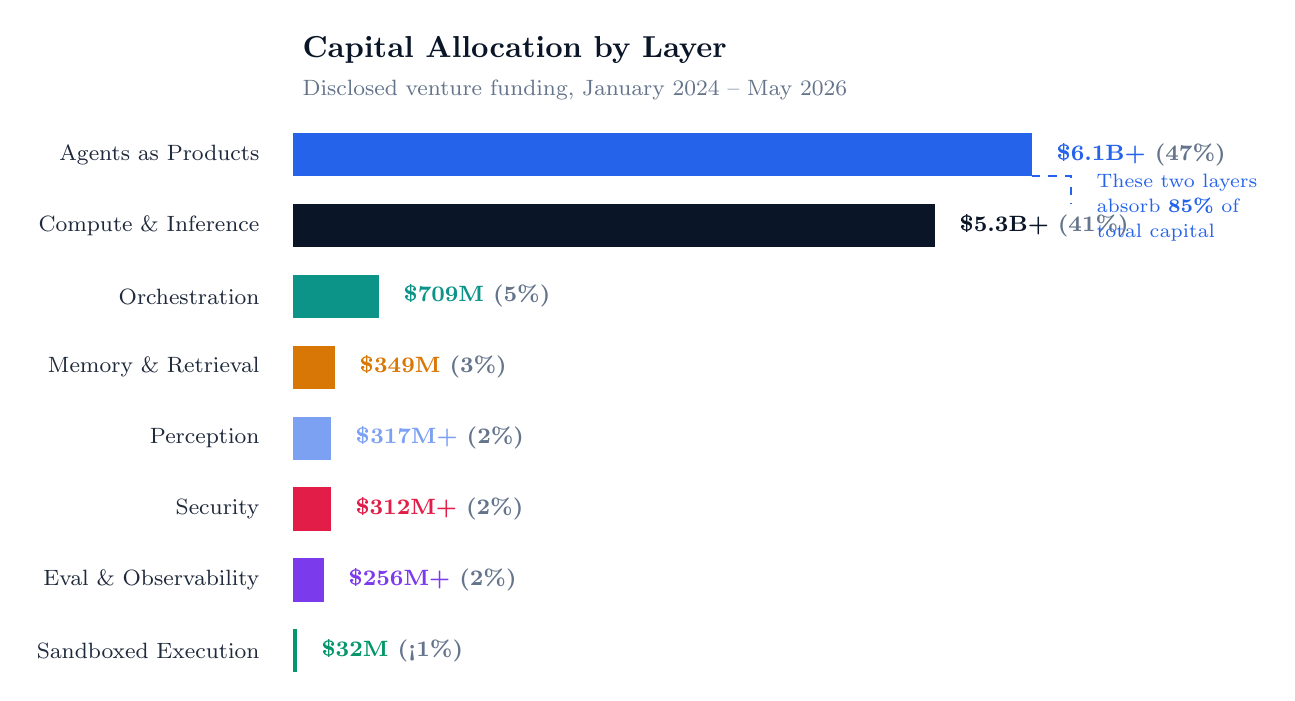
\begin{tikzpicture}

% Title
\node[anchor=west, font=\fontsize{11}{13}\selectfont\bfseries\color{navy}] at (0, 5.8) {Capital Allocation by Layer};
\node[anchor=west, font=\fontsize{8.5}{10}\selectfont\color{textsub}] at (0, 5.3) {Disclosed venture funding, January 2024 -- May 2026};

% Horizontal bar chart
\def\barheight{0.55}
\def\maxwidth{10}

% Agents as Products - $6.1B (47%)
\fill[primary] (0, 4.2) rectangle ({6.1/6.5*\maxwidth}, 4.2+\barheight);
\node[anchor=east, font=\fontsize{8.5}{10}\selectfont\color{textmain}] at (-0.3, 4.2+\barheight/2) {Agents as Products};
\node[anchor=west, font=\fontsize{8.5}{10}\selectfont\bfseries\color{primary}] at ({6.1/6.5*\maxwidth+0.2}, 4.2+\barheight/2) {\$6.1B+ {\footnotesize\color{textsub}(47\%)}};

% Compute - $5.3B (41%)
\fill[navy] (0, 3.3) rectangle ({5.3/6.5*\maxwidth}, 3.3+\barheight);
\node[anchor=east, font=\fontsize{8.5}{10}\selectfont\color{textmain}] at (-0.3, 3.3+\barheight/2) {Compute \& Inference};
\node[anchor=west, font=\fontsize{8.5}{10}\selectfont\bfseries\color{navy}] at ({5.3/6.5*\maxwidth+0.2}, 3.3+\barheight/2) {\$5.3B+ {\footnotesize\color{textsub}(41\%)}};

% Orchestration - $709M (5%)
\fill[chartteal] (0, 2.4) rectangle ({0.709/6.5*\maxwidth}, 2.4+\barheight);
\node[anchor=east, font=\fontsize{8.5}{10}\selectfont\color{textmain}] at (-0.3, 2.4+\barheight/2) {Orchestration};
\node[anchor=west, font=\fontsize{8.5}{10}\selectfont\bfseries\color{chartteal}] at ({0.709/6.5*\maxwidth+0.2}, 2.4+\barheight/2) {\$709M {\footnotesize\color{textsub}(5\%)}};

% Memory - $349M (3%)
\fill[chartamber] (0, 1.5) rectangle ({0.349/6.5*\maxwidth}, 1.5+\barheight);
\node[anchor=east, font=\fontsize{8.5}{10}\selectfont\color{textmain}] at (-0.3, 1.5+\barheight/2) {Memory \& Retrieval};
\node[anchor=west, font=\fontsize{8.5}{10}\selectfont\bfseries\color{chartamber}] at ({0.349/6.5*\maxwidth+0.2}, 1.5+\barheight/2) {\$349M {\footnotesize\color{textsub}(3\%)}};

% Perception - $317M (2%)
\fill[primary!60] (0, 0.6) rectangle ({0.317/6.5*\maxwidth}, 0.6+\barheight);
\node[anchor=east, font=\fontsize{8.5}{10}\selectfont\color{textmain}] at (-0.3, 0.6+\barheight/2) {Perception};
\node[anchor=west, font=\fontsize{8.5}{10}\selectfont\bfseries\color{primary!60}] at ({0.317/6.5*\maxwidth+0.2}, 0.6+\barheight/2) {\$317M+ {\footnotesize\color{textsub}(2\%)}};

% Security - $312M (2%)
\fill[chartrose] (0, -0.3) rectangle ({0.312/6.5*\maxwidth}, -0.3+\barheight);
\node[anchor=east, font=\fontsize{8.5}{10}\selectfont\color{textmain}] at (-0.3, -0.3+\barheight/2) {Security};
\node[anchor=west, font=\fontsize{8.5}{10}\selectfont\bfseries\color{chartrose}] at ({0.312/6.5*\maxwidth+0.2}, -0.3+\barheight/2) {\$312M+ {\footnotesize\color{textsub}(2\%)}};

% Eval - $256M (2%)
\fill[chartpurple] (0, -1.2) rectangle ({0.256/6.5*\maxwidth}, -1.2+\barheight);
\node[anchor=east, font=\fontsize{8.5}{10}\selectfont\color{textmain}] at (-0.3, -1.2+\barheight/2) {Eval \& Observability};
\node[anchor=west, font=\fontsize{8.5}{10}\selectfont\bfseries\color{chartpurple}] at ({0.256/6.5*\maxwidth+0.2}, -1.2+\barheight/2) {\$256M+ {\footnotesize\color{textsub}(2\%)}};

% Sandboxed - $32M (<1%)
\fill[success] (0, -2.1) rectangle ({0.032/6.5*\maxwidth}, -2.1+\barheight);
\node[anchor=east, font=\fontsize{8.5}{10}\selectfont\color{textmain}] at (-0.3, -2.1+\barheight/2) {Sandboxed Execution};
\node[anchor=west, font=\fontsize{8.5}{10}\selectfont\bfseries\color{success}] at ({0.032/6.5*\maxwidth+0.2}, -2.1+\barheight/2) {\$32M {\footnotesize\color{textsub}({<}1\%)}};

% Annotation callout
\draw[primary, line width=0.8pt, dashed] ({6.1/6.5*\maxwidth}, 4.2) -- ({6.1/6.5*\maxwidth+0.5}, 4.2) -- ({6.1/6.5*\maxwidth+0.5}, 3.3+\barheight);
\node[anchor=west, font=\fontsize{7.5}{9}\selectfont\color{primary}, align=left] at ({6.1/6.5*\maxwidth+0.7}, 3.8) {These two layers\\absorb \textbf{85\%} of\\total capital};

\end{tikzpicture}

\vspace{10mm}

% ─── Revenue Multiples Callout ───
\noindent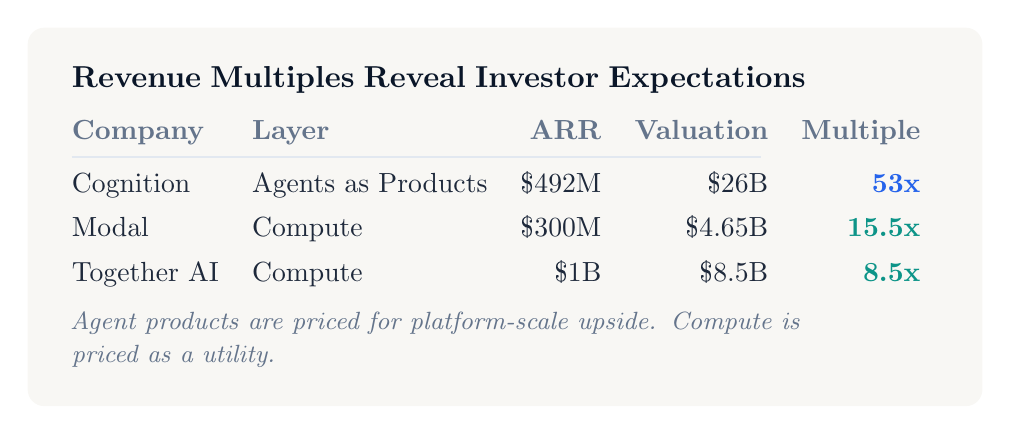
\begin{tikzpicture}
\node[
  rectangle, rounded corners=6pt,
  fill=warmgray,
  minimum width=\textwidth,
  inner sep=14pt,
  text width=\textwidth-32pt,
] {
  \begin{minipage}{\textwidth-32pt}
  {\fontsize{11}{13}\selectfont\bfseries\color{navy}Revenue Multiples Reveal Investor Expectations}\\[6pt]
  {\fontsize{10}{14}\selectfont\color{textmain}
  \begin{tabularx}{\textwidth-32pt}{@{} l l r r r @{}}
  \arrayrulecolor{tableborder}
  \textbf{\color{textsub}Company} & \textbf{\color{textsub}Layer} & \textbf{\color{textsub}ARR} & \textbf{\color{textsub}Valuation} & \textbf{\color{textsub}Multiple} \\
  \midrule
  Cognition & Agents as Products & \$492M & \$26B & {\bfseries\color{primary}53x} \\[2pt]
  Modal & Compute & \$300M & \$4.65B & {\bfseries\color{chartteal}15.5x} \\[2pt]
  Together AI & Compute & \$1B & \$8.5B & {\bfseries\color{chartteal}8.5x} \\[2pt]
  \end{tabularx}
  
  \vspace{4pt}
  {\fontsize{9}{11}\selectfont\color{textsub}\textit{Agent products are priced for platform-scale upside. Compute is priced as a utility.}}
  }
  \end{minipage}
};
\end{tikzpicture}

\clearpage


% ─── FUNDING VELOCITY PAGE ───

\subsection*{Funding Velocity}

\vspace{4mm}

\noindent\hfill
\statbox{48mm}{\$1.5B}{2024 Funding}
\hfill
\statbox{48mm}{\$2.9B}{2025 Funding}
\hfill
\statbox{48mm}{\raisebox{0pt}{\fontsize{22}{26}\selectfont$\sim$}\$2.6B}{2026 Annualized}
\hfill\null

\vspace{10mm}

% Funding growth chart
\noindent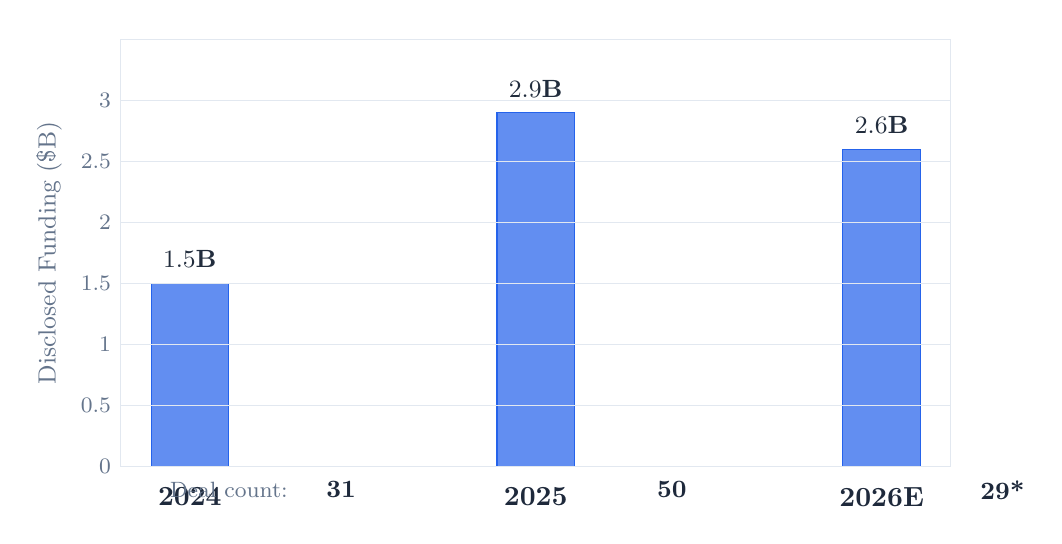
\begin{tikzpicture}
  \begin{axis}[
    width=\textwidth,
    height=7cm,
    ybar,
    bar width=28pt,
    ymin=0, ymax=3.5,
    xtick=data,
    xticklabels={2024, 2025, 2026E},
    ylabel={Disclosed Funding (\$B)},
    ylabel style={font=\fontsize{9}{11}\selectfont\color{textsub}},
    xticklabel style={font=\fontsize{10}{12}\selectfont\bfseries\color{textmain}},
    yticklabel style={font=\fontsize{8}{10}\selectfont\color{textsub}},
    ytick={0, 0.5, 1.0, 1.5, 2.0, 2.5, 3.0},
    axis line style={draw=tableborder},
    tick style={draw=none},
    ymajorgrids=true,
    grid style={draw=tableborder, line width=0.3pt},
    axis on top,
    nodes near coords={\pgfmathprintnumber\pgfplotspointmeta B},
    nodes near coords style={font=\fontsize{9}{11}\selectfont\bfseries\color{navy}, above=2pt},
    every axis plot/.append style={fill opacity=0.9},
  ]
  \addplot[fill=primary!80, draw=primary] coordinates {(1,1.5) (2,2.9) (3,2.6)};
  \end{axis}
  
  % Deal count annotation
  \node[anchor=west, font=\fontsize{8}{10}\selectfont\color{textsub}] at (0.5, -0.3) {Deal count:};
  \node[anchor=center, font=\fontsize{9}{11}\selectfont\bfseries\color{textmain}] at (2.8, -0.3) {31};
  \node[anchor=center, font=\fontsize{9}{11}\selectfont\bfseries\color{textmain}] at (7.0, -0.3) {50};
  \node[anchor=center, font=\fontsize{9}{11}\selectfont\bfseries\color{textmain}] at (11.2, -0.3) {29*};
  
\end{tikzpicture}

\vspace{2mm}
{\fontsize{8.5}{10}\selectfont\color{textsub}\textit{*Jan--May 2026 only. Annualized figure assumes linear pace. Source: Author's dataset from Crunchbase, PitchBook, and media reports.}}

\vspace{10mm}

% ─── Enterprise Readiness Gap ───
\subsection*{The Enterprise Readiness Gap}

\vspace{4mm}

\noindent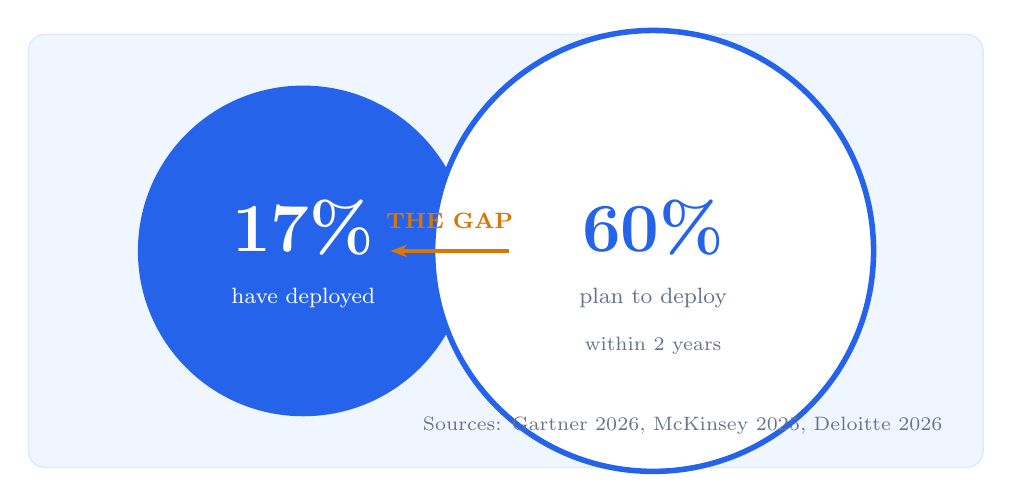
\begin{tikzpicture}
  % Container
  \node[rectangle, rounded corners=6pt, fill=lightbluebg, draw=lightblue, line width=0.5pt,
    minimum width=\textwidth, minimum height=55mm, inner sep=0pt] (container) {};
  
  % Left: 17% deployed circle
  \node[circle, fill=primary, minimum size=42mm, inner sep=0pt] (deployed) at ([xshift=35mm, yshift=0mm]container.west) {};
  \node[font=\fontsize{30}{34}\selectfont\bfseries, text=white] at ([yshift=3mm]deployed.center) {17\%};
  \node[font=\fontsize{8.5}{10}\selectfont, text=white] at ([yshift=-6mm]deployed.center) {have deployed};
  
  % Right: 60% planning circle
  \node[circle, draw=primary, line width=2pt, fill=white, minimum size=56mm, inner sep=0pt] (planning) at ([xshift=-42mm, yshift=0mm]container.east) {};
  \node[font=\fontsize{30}{34}\selectfont\bfseries, text=primary] at ([yshift=3mm]planning.center) {60\%};
  \node[font=\fontsize{8.5}{10}\selectfont, text=textsub] at ([yshift=-6mm]planning.center) {plan to deploy};
  \node[font=\fontsize{7.5}{9}\selectfont, text=textsub] at ([yshift=-12mm]planning.center) {within 2 years};
  
  % Arrow between
  \draw[-{Stealth[length=6pt]}, line width=1.5pt, warning] ([xshift=5mm]deployed.east) -- ([xshift=-5mm]planning.west) node[midway, above=4pt, font=\fontsize{8}{10}\selectfont\bfseries\color{warning}] {THE GAP};
  
  % Source
  \node[anchor=south east, font=\fontsize{7}{9}\selectfont\color{textsub}] at ([xshift=-4mm, yshift=3mm]container.south east) {Sources: Gartner 2026, McKinsey 2025, Deloitte 2026};
  
\end{tikzpicture}

\vspace{4mm}

\pullquote{This combination of high intent, low maturity, and minimal governance creates the demand that infrastructure companies fill.}


\clearpage


% ═══════════════════════════════════
% SECTION 3: ARCHITECTURAL TRENDS
% ═══════════════════════════════════
\sectionbanner{03}{Six Architectural Trends}

{\fontsize{10.5}{15}\selectfont
Six architectural trends are reshaping how developers build and deploy agents. Each represents a shift from pre-agent to agent-first infrastructure design.
}

\vspace{8mm}

% ─── Trends Grid ───
\noindent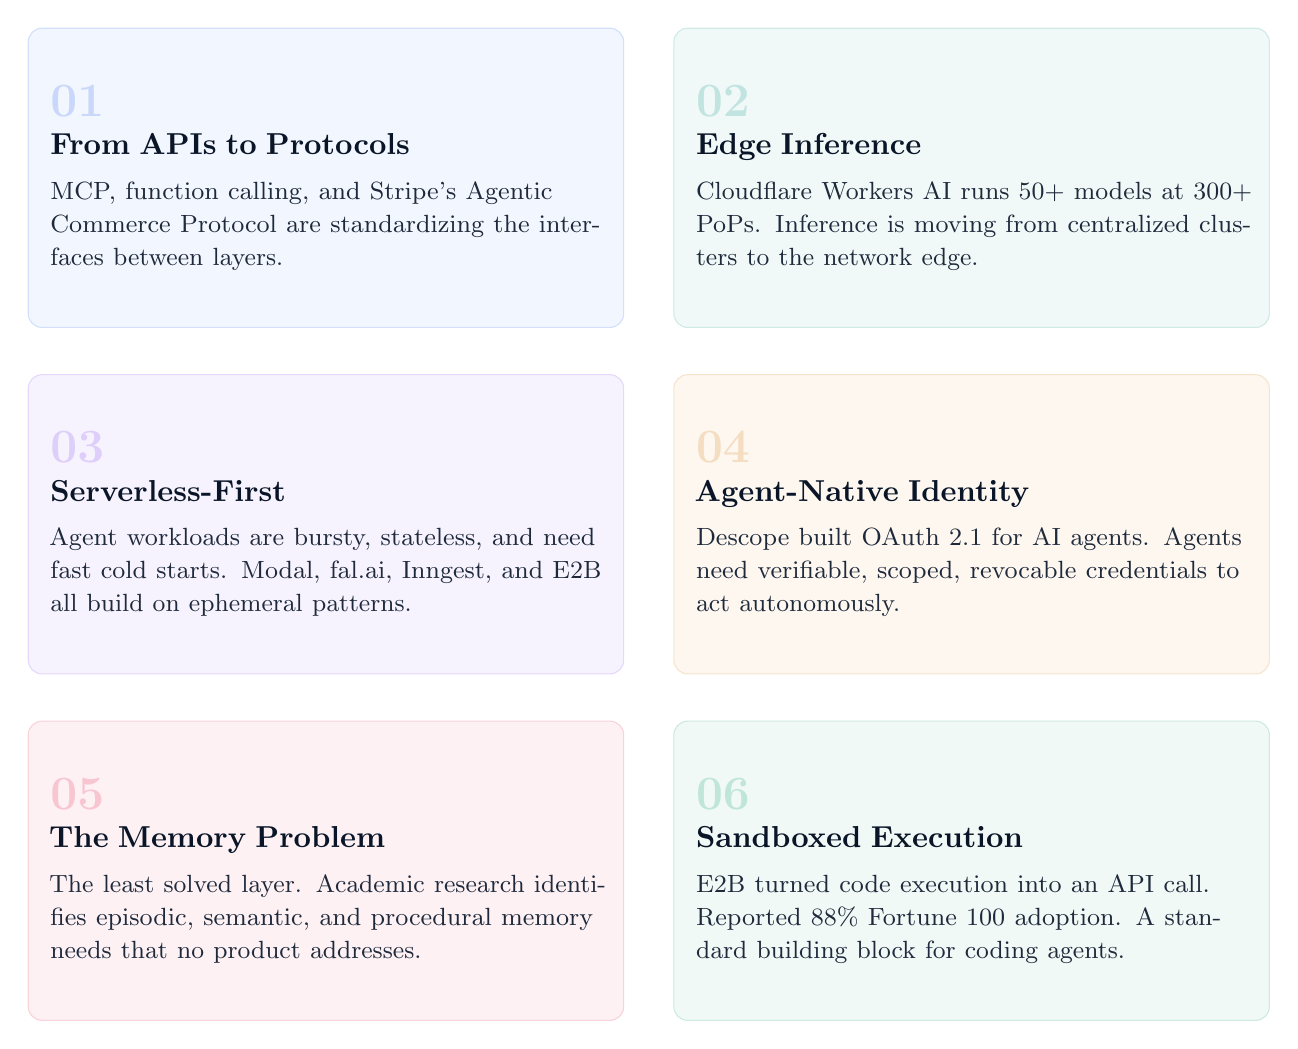
\begin{tikzpicture}[
  trendbox/.style={
    rectangle, rounded corners=5pt,
    minimum width=75mm, minimum height=38mm,
    inner sep=8pt, text width=70mm,
    anchor=north west,
  },
]

% Row 1
\node[trendbox, fill=primary!6, draw=primary!20] (t1) at (0, 0) {
  {\fontsize{18}{20}\selectfont\color{primary!25}\bfseries 01}\\[2pt]
  {\fontsize{11}{13}\selectfont\bfseries\color{navy}From APIs to Protocols}\\[4pt]
  {\fontsize{9}{12}\selectfont\color{textmain}MCP, function calling, and Stripe's Agentic Commerce Protocol are standardizing the interfaces between layers.}
};

\node[trendbox, fill=chartteal!6, draw=chartteal!20] (t2) at (82mm, 0) {
  {\fontsize{18}{20}\selectfont\color{chartteal!25}\bfseries 02}\\[2pt]
  {\fontsize{11}{13}\selectfont\bfseries\color{navy}Edge Inference}\\[4pt]
  {\fontsize{9}{12}\selectfont\color{textmain}Cloudflare Workers AI runs 50+ models at 300+ PoPs. Inference is moving from centralized clusters to the network edge.}
};

% Row 2
\node[trendbox, fill=chartpurple!6, draw=chartpurple!20] (t3) at (0, -44mm) {
  {\fontsize{18}{20}\selectfont\color{chartpurple!25}\bfseries 03}\\[2pt]
  {\fontsize{11}{13}\selectfont\bfseries\color{navy}Serverless-First}\\[4pt]
  {\fontsize{9}{12}\selectfont\color{textmain}Agent workloads are bursty, stateless, and need fast cold starts. Modal, fal.ai, Inngest, and E2B all build on ephemeral patterns.}
};

\node[trendbox, fill=chartamber!6, draw=chartamber!20] (t4) at (82mm, -44mm) {
  {\fontsize{18}{20}\selectfont\color{chartamber!25}\bfseries 04}\\[2pt]
  {\fontsize{11}{13}\selectfont\bfseries\color{navy}Agent-Native Identity}\\[4pt]
  {\fontsize{9}{12}\selectfont\color{textmain}Descope built OAuth 2.1 for AI agents. Agents need verifiable, scoped, revocable credentials to act autonomously.}
};

% Row 3
\node[trendbox, fill=chartrose!6, draw=chartrose!20] (t5) at (0, -88mm) {
  {\fontsize{18}{20}\selectfont\color{chartrose!25}\bfseries 05}\\[2pt]
  {\fontsize{11}{13}\selectfont\bfseries\color{navy}The Memory Problem}\\[4pt]
  {\fontsize{9}{12}\selectfont\color{textmain}The least solved layer. Academic research identifies episodic, semantic, and procedural memory needs that no product addresses.}
};

\node[trendbox, fill=success!6, draw=success!20] (t6) at (82mm, -88mm) {
  {\fontsize{18}{20}\selectfont\color{success!25}\bfseries 06}\\[2pt]
  {\fontsize{11}{13}\selectfont\bfseries\color{navy}Sandboxed Execution}\\[4pt]
  {\fontsize{9}{12}\selectfont\color{textmain}E2B turned code execution into an API call. Reported 88\% Fortune 100 adoption. A standard building block for coding agents.}
};

\end{tikzpicture}


\clearpage

% ═══════════════════════════════════
% SECTION 4: CONSOLIDATION
% ═══════════════════════════════════
\sectionbanner{04}{Consolidation Dynamics}

{\fontsize{10.5}{15}\selectfont
Eight acquisitions occurred between September 2024 and May 2026. The acquirers share a consistent profile: large infrastructure incumbents that missed the initial agent wave and bought their way in.
}

\vspace{8mm}

% ─── Acquisition Timeline ───
\noindent\begin{tikzpicture}

\node[anchor=west, font=\fontsize{11}{13}\selectfont\bfseries\color{navy}] at (0, 6) {Agent Infrastructure Acquisitions};

% Timeline line
\draw[navy, line width=1.5pt] (0, 4.8) -- (\textwidth, 4.8);

% Timeline ticks and events
\def\tw{\textwidth}

% Sep 2024 - Cisco/Robust Intelligence
\fill[primary] (0.5, 4.8) circle (4pt);
\node[anchor=north, font=\fontsize{7.5}{9}\selectfont\color{textsub}, align=center] at (0.5, 4.4) {Sep 2024};
\node[anchor=south, font=\fontsize{8}{10}\selectfont\color{textmain}, align=center, text width=22mm] at (0.5, 5.2) {\textbf{Cisco} acquires\\Robust Int.};

% Feb 2025 - IBM/HashiCorp
\fill[navy] (3.2, 4.8) circle (4pt);
\node[anchor=north, font=\fontsize{7.5}{9}\selectfont\color{textsub}, align=center] at (3.2, 4.4) {Feb 2025};
\node[anchor=south, font=\fontsize{8}{10}\selectfont\color{textmain}, align=center, text width=22mm] at (3.2, 5.2) {\textbf{IBM} acquires\\HashiCorp\\\footnotesize\$6.4B};

% Sep 2025 - Check Point/Lakera
\fill[chartrose] (5.9, 4.8) circle (4pt);
\node[anchor=north, font=\fontsize{7.5}{9}\selectfont\color{textsub}, align=center] at (5.9, 4.4) {Sep 2025};
\node[anchor=south, font=\fontsize{8}{10}\selectfont\color{textmain}, align=center, text width=24mm] at (5.9, 5.2) {\textbf{Check Point}\\acquires Lakera\\\footnotesize\raisebox{0pt}{\~{}}\$300M};

% Dec 2025 - Meta/Manus (blocked)
\fill[warning] (7.6, 4.8) circle (4pt);
\node[anchor=north, font=\fontsize{7.5}{9}\selectfont\color{textsub}, align=center] at (7.6, 4.4) {Dec 2025};
\node[anchor=south, font=\fontsize{8}{10}\selectfont\color{textmain}, align=center, text width=22mm] at (7.6, 5.2) {\textbf{Meta}/Manus\\\footnotesize\raisebox{0pt}{\~{}}\$2B\\\footnotesize\color{danger}(blocked)};

% Jan 2026 - ClickHouse/Langfuse
\fill[chartpurple] (9.3, 4.8) circle (4pt);
\node[anchor=north, font=\fontsize{7.5}{9}\selectfont\color{textsub}, align=center] at (9.3, 4.4) {Jan 2026};
\node[anchor=south, font=\fontsize{8}{10}\selectfont\color{textmain}, align=center, text width=24mm] at (9.3, 5.2) {\textbf{ClickHouse}\\acquires Langfuse};

% Mar 2026 - Mintlify/Helicone + IBM/Confluent
\fill[chartteal] (11.5, 4.8) circle (4pt);
\node[anchor=north, font=\fontsize{7.5}{9}\selectfont\color{textsub}, align=center, text width=28mm] at (11.5, 4.4) {Mar 2026};
\node[anchor=south, font=\fontsize{8}{10}\selectfont\color{textmain}, align=center, text width=28mm] at (11.5, 5.2) {\textbf{IBM}/Confluent\\\footnotesize\$11B\\+ Mintlify/Helicone};

% Apr 2026 - Cisco/Galileo
\fill[primary] (13.5, 4.8) circle (4pt);
\node[anchor=north, font=\fontsize{7.5}{9}\selectfont\color{textsub}, align=center] at (13.5, 4.4) {Apr 2026};
\node[anchor=south, font=\fontsize{8}{10}\selectfont\color{textmain}, align=center, text width=22mm] at (13.5, 5.2) {\textbf{Cisco} acquires\\Galileo AI};

% Legend
\node[anchor=west, font=\fontsize{7.5}{9}\selectfont\color{textsub}] at (0, 3.4) {
  \tikz\fill[primary] (0,0) circle (3pt); Security \hspace{6pt}
  \tikz\fill[chartpurple] (0,0) circle (3pt); Observability \hspace{6pt}
  \tikz\fill[navy] (0,0) circle (3pt); Adjacent infra \hspace{6pt}
  \tikz\fill[warning] (0,0) circle (3pt); Blocked deal
};

\end{tikzpicture}

\vspace{8mm}

% ─── What Gets Acquired vs Independent ───
\noindent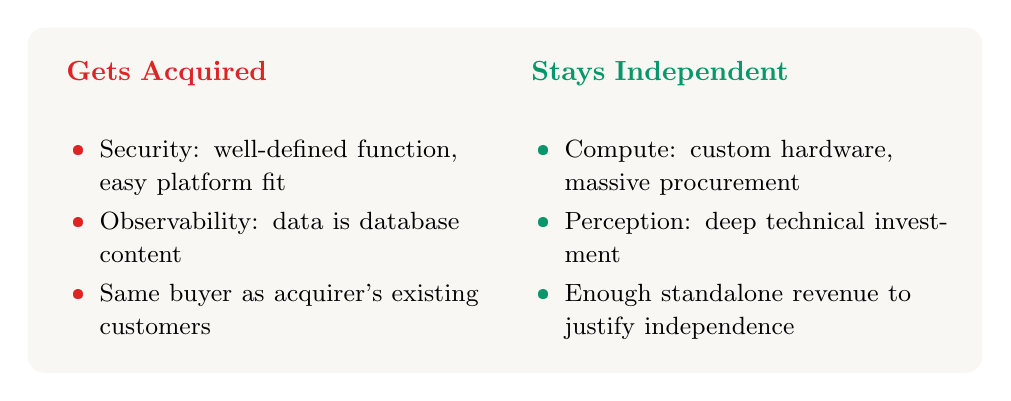
\begin{tikzpicture}
\node[rectangle, rounded corners=6pt, fill=warmgray, minimum width=\textwidth, inner sep=12pt, text width=\textwidth-28pt] {
  \begin{minipage}[t]{0.47\textwidth}
    {\fontsize{10}{12}\selectfont\bfseries\color{danger}Gets Acquired}\\[4pt]
    \begin{itemize}[leftmargin=12pt, itemsep=2pt, parsep=0pt]
      \item[\color{danger}\textbullet] {\fontsize{9}{12}\selectfont Security: well-defined function, easy platform fit}
      \item[\color{danger}\textbullet] {\fontsize{9}{12}\selectfont Observability: data is database content}
      \item[\color{danger}\textbullet] {\fontsize{9}{12}\selectfont Same buyer as acquirer's existing customers}
    \end{itemize}
  \end{minipage}%
  \hfill
  \begin{minipage}[t]{0.47\textwidth}
    {\fontsize{10}{12}\selectfont\bfseries\color{success}Stays Independent}\\[4pt]
    \begin{itemize}[leftmargin=12pt, itemsep=2pt, parsep=0pt]
      \item[\color{success}\textbullet] {\fontsize{9}{12}\selectfont Compute: custom hardware, massive procurement}
      \item[\color{success}\textbullet] {\fontsize{9}{12}\selectfont Perception: deep technical investment}
      \item[\color{success}\textbullet] {\fontsize{9}{12}\selectfont Enough standalone revenue to justify independence}
    \end{itemize}
  \end{minipage}
};
\end{tikzpicture}


\clearpage


% ═══════════════════════════════════
% SECTION 5: PLATFORM CONVERGENCE
% ═══════════════════════════════════
\sectionbanner{05}{Platform Convergence}

{\fontsize{10.5}{15}\selectfont
Three platform convergence patterns are pulling standalone tools into unified marketplaces, mirroring the decade-long AWS absorption cycle in compressed form.
}

\vspace{8mm}

% ─── Platform Vulnerability Table ───
\noindent
\begin{tikzpicture}
\node[anchor=west, font=\fontsize{11}{13}\selectfont\bfseries\color{navy}] at (0, 0.3) {Layer Vulnerability to Platform Absorption};
\end{tikzpicture}

\vspace{4mm}

\renewcommand{\arraystretch}{1.6}
\noindent\begin{tabularx}{\textwidth}{@{} >{\centering\arraybackslash}p{24mm} X >{\raggedright\arraybackslash}p{52mm} @{}}
\arrayrulecolor{tableborder}
\rowcolor{navy} \textbf{\color{white}\fontsize{8.5}{10}\selectfont Vulnerability} & \textbf{\color{white}\fontsize{8.5}{10}\selectfont Layers} & \textbf{\color{white}\fontsize{8.5}{10}\selectfont Signal} \\
\rowcolor{danger!8} {\fontsize{9}{11}\selectfont\bfseries\color{danger}HIGH} & {\fontsize{9.5}{12}\selectfont Security, Observability} & {\fontsize{8.5}{11}\selectfont Already being acquired. Feature-like scope.} \\
\rowcolor{warning!8} {\fontsize{9}{11}\selectfont\bfseries\color{warning}MEDIUM} & {\fontsize{9.5}{12}\selectfont Memory, Orchestration} & {\fontsize{8.5}{11}\selectfont Databases adding vector search. Cloud adding workflows.} \\
\rowcolor{success!8} {\fontsize{9}{11}\selectfont\bfseries\color{success}LOW} & {\fontsize{9.5}{12}\selectfont Compute, Perception} & {\fontsize{8.5}{11}\selectfont Custom hardware and deep technical barriers.} \\
\rowcolor{primary!5} {\fontsize{9}{11}\selectfont\bfseries\color{primary}SPECIAL} & {\fontsize{9.5}{12}\selectfont Sandboxed Execution} & {\fontsize{8.5}{11}\selectfont Narrow function. Single-company layer.} \\
\end{tabularx}

\vspace{12mm}

% ─── Investor Thesis Orientations ───
\subsection*{Investor Thesis Orientations}

\vspace{4mm}

\noindent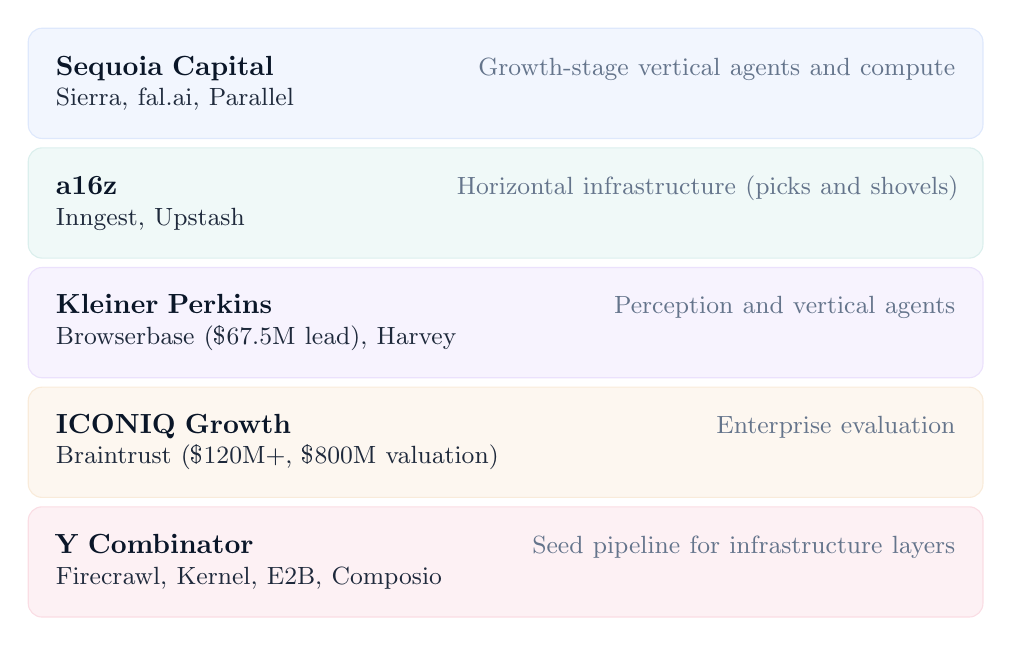
\begin{tikzpicture}[
  investorbox/.style={
    rectangle, rounded corners=5pt,
    minimum width=\textwidth, minimum height=14mm,
    inner sep=8pt, text width=\textwidth-20pt,
  },
]

\node[investorbox, fill=primary!6, draw=primary!15] (i1) at (0, 0) {
  {\fontsize{10}{12}\selectfont\bfseries\color{navy}Sequoia Capital} \hfill {\fontsize{9}{11}\selectfont\color{textsub}Growth-stage vertical agents and compute}\\[-1pt]
  {\fontsize{9}{11}\selectfont\color{textmain}Sierra, fal.ai, Parallel}
};

\node[investorbox, fill=chartteal!6, draw=chartteal!15, below=3pt of i1] (i2) {
  {\fontsize{10}{12}\selectfont\bfseries\color{navy}a16z} \hfill {\fontsize{9}{11}\selectfont\color{textsub}Horizontal infrastructure (picks and shovels)}\\[-1pt]
  {\fontsize{9}{11}\selectfont\color{textmain}Inngest, Upstash}
};

\node[investorbox, fill=chartpurple!6, draw=chartpurple!15, below=3pt of i2] (i3) {
  {\fontsize{10}{12}\selectfont\bfseries\color{navy}Kleiner Perkins} \hfill {\fontsize{9}{11}\selectfont\color{textsub}Perception and vertical agents}\\[-1pt]
  {\fontsize{9}{11}\selectfont\color{textmain}Browserbase (\$67.5M lead), Harvey}
};

\node[investorbox, fill=chartamber!6, draw=chartamber!15, below=3pt of i3] (i4) {
  {\fontsize{10}{12}\selectfont\bfseries\color{navy}ICONIQ Growth} \hfill {\fontsize{9}{11}\selectfont\color{textsub}Enterprise evaluation}\\[-1pt]
  {\fontsize{9}{11}\selectfont\color{textmain}Braintrust (\$120M+, \$800M valuation)}
};

\node[investorbox, fill=chartrose!6, draw=chartrose!15, below=3pt of i4] (i5) {
  {\fontsize{10}{12}\selectfont\bfseries\color{navy}Y Combinator} \hfill {\fontsize{9}{11}\selectfont\color{textsub}Seed pipeline for infrastructure layers}\\[-1pt]
  {\fontsize{9}{11}\selectfont\color{textmain}Firecrawl, Kernel, E2B, Composio}
};

\end{tikzpicture}


\clearpage


% ═══════════════════════════════════
% SECTION 6: OPEN QUESTIONS AND OUTLOOK
% ═══════════════════════════════════
\sectionbanner{07}{Open Questions and Outlook}

\vspace{4mm}

{\fontsize{10.5}{15}\selectfont
The eight-layer structure is transitional. The evidence in this paper points toward consolidation from eight layers to approximately five within three years.
}

\vspace{8mm}

% ─── Consolidation Forecast ───
\noindent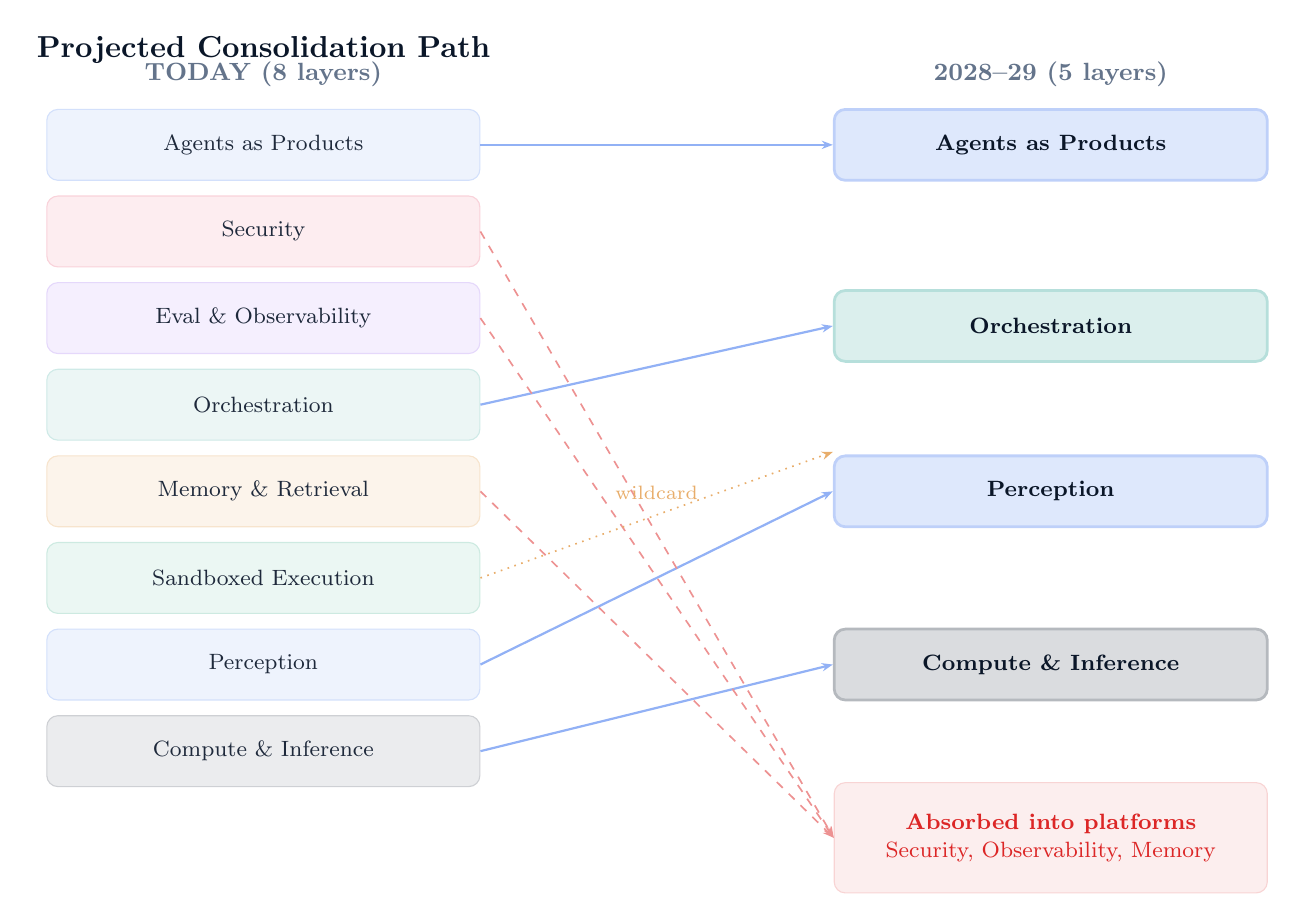
\begin{tikzpicture}

\node[anchor=west, font=\fontsize{11}{13}\selectfont\bfseries\color{navy}] at (0, 0) {Projected Consolidation Path};

% Today column
\node[rectangle, rounded corners=4pt, fill=primary!8, draw=primary!20, minimum width=55mm, minimum height=9mm, inner sep=4pt, font=\fontsize{8.5}{10}\selectfont\color{textmain}, align=center] (t1) at (30mm, -12mm) {Agents as Products};
\node[rectangle, rounded corners=4pt, fill=chartrose!8, draw=chartrose!20, minimum width=55mm, minimum height=9mm, inner sep=4pt, font=\fontsize{8.5}{10}\selectfont\color{textmain}, align=center] (t2) at (30mm, -23mm) {Security};
\node[rectangle, rounded corners=4pt, fill=chartpurple!8, draw=chartpurple!20, minimum width=55mm, minimum height=9mm, inner sep=4pt, font=\fontsize{8.5}{10}\selectfont\color{textmain}, align=center] (t3) at (30mm, -34mm) {Eval \& Observability};
\node[rectangle, rounded corners=4pt, fill=chartteal!8, draw=chartteal!20, minimum width=55mm, minimum height=9mm, inner sep=4pt, font=\fontsize{8.5}{10}\selectfont\color{textmain}, align=center] (t4) at (30mm, -45mm) {Orchestration};
\node[rectangle, rounded corners=4pt, fill=chartamber!8, draw=chartamber!20, minimum width=55mm, minimum height=9mm, inner sep=4pt, font=\fontsize{8.5}{10}\selectfont\color{textmain}, align=center] (t5) at (30mm, -56mm) {Memory \& Retrieval};
\node[rectangle, rounded corners=4pt, fill=success!8, draw=success!20, minimum width=55mm, minimum height=9mm, inner sep=4pt, font=\fontsize{8.5}{10}\selectfont\color{textmain}, align=center] (t6) at (30mm, -67mm) {Sandboxed Execution};
\node[rectangle, rounded corners=4pt, fill=primary!8, draw=primary!20, minimum width=55mm, minimum height=9mm, inner sep=4pt, font=\fontsize{8.5}{10}\selectfont\color{textmain}, align=center] (t7) at (30mm, -78mm) {Perception};
\node[rectangle, rounded corners=4pt, fill=navy!8, draw=navy!20, minimum width=55mm, minimum height=9mm, inner sep=4pt, font=\fontsize{8.5}{10}\selectfont\color{textmain}, align=center] (t8) at (30mm, -89mm) {Compute \& Inference};

% Column labels
\node[font=\fontsize{9}{11}\selectfont\bfseries\color{textsub}] at (30mm, -3mm) {TODAY (8 layers)};
\node[font=\fontsize{9}{11}\selectfont\bfseries\color{textsub}] at (130mm, -3mm) {2028--29 (5 layers)};

% Future column
\node[rectangle, rounded corners=4pt, fill=primary!15, draw=primary!30, line width=1pt, minimum width=55mm, minimum height=9mm, inner sep=4pt, font=\fontsize{8.5}{10}\selectfont\bfseries\color{navy}, align=center] (f1) at (130mm, -12mm) {Agents as Products};
\node[rectangle, rounded corners=4pt, fill=chartteal!15, draw=chartteal!30, line width=1pt, minimum width=55mm, minimum height=9mm, inner sep=4pt, font=\fontsize{8.5}{10}\selectfont\bfseries\color{navy}, align=center] (f2) at (130mm, -35mm) {Orchestration};
\node[rectangle, rounded corners=4pt, fill=primary!15, draw=primary!30, line width=1pt, minimum width=55mm, minimum height=9mm, inner sep=4pt, font=\fontsize{8.5}{10}\selectfont\bfseries\color{navy}, align=center] (f3) at (130mm, -56mm) {Perception};
\node[rectangle, rounded corners=4pt, fill=navy!15, draw=navy!30, line width=1pt, minimum width=55mm, minimum height=9mm, inner sep=4pt, font=\fontsize{8.5}{10}\selectfont\bfseries\color{navy}, align=center] (f4) at (130mm, -78mm) {Compute \& Inference};

% "Absorbed into platforms" label
\node[rectangle, rounded corners=4pt, fill=danger!8, draw=danger!20, minimum width=55mm, minimum height=14mm, inner sep=4pt, font=\fontsize{8}{10}\selectfont\color{danger}, align=center] (abs) at (130mm, -100mm) {\textbf{Absorbed into platforms}\\Security, Observability, Memory};

% Arrows
\draw[-{Stealth[length=4pt]}, primary!50, line width=0.8pt] (t1.east) -- (f1.west);
\draw[-{Stealth[length=4pt]}, primary!50, line width=0.8pt] (t4.east) -- (f2.west);
\draw[-{Stealth[length=4pt]}, primary!50, line width=0.8pt] (t7.east) -- (f3.west);
\draw[-{Stealth[length=4pt]}, primary!50, line width=0.8pt] (t8.east) -- (f4.west);

% Absorbed arrows
\draw[-{Stealth[length=4pt]}, danger!50, line width=0.6pt, dashed] (t2.east) -- (abs.west);
\draw[-{Stealth[length=4pt]}, danger!50, line width=0.6pt, dashed] (t3.east) -- (abs.west);
\draw[-{Stealth[length=4pt]}, danger!50, line width=0.6pt, dashed] (t5.east) -- (abs.west);

% Wildcard
\draw[-{Stealth[length=4pt]}, warning!60, line width=0.6pt, dotted] (t6.east) -- ([yshift=5mm]f3.west) node[midway, above=2pt, font=\fontsize{7}{9}\selectfont\color{warning}] {wildcard};

\end{tikzpicture}

\vspace{10mm}

% ─── Key Risks ───
\subsection*{Key Risks}

\vspace{4mm}

\noindent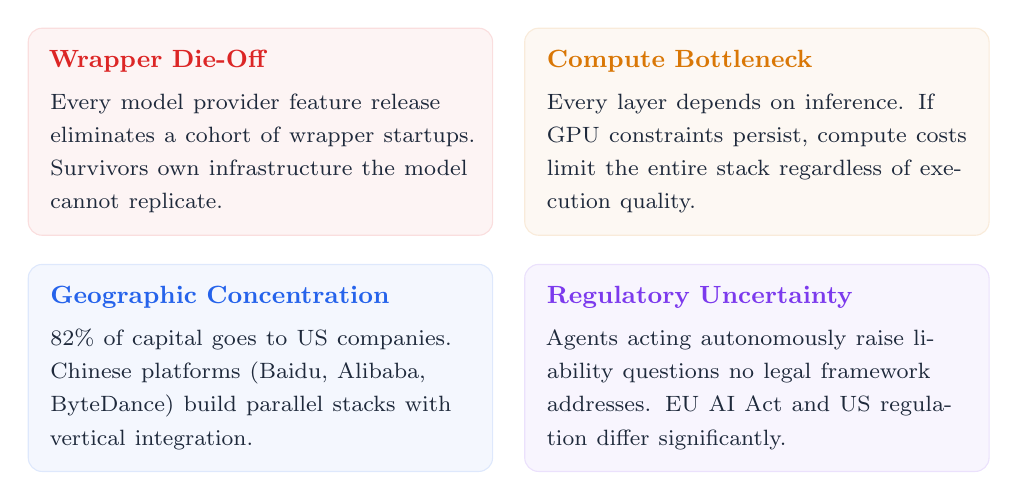
\begin{tikzpicture}[
  riskbox/.style={
    rectangle, rounded corners=5pt,
    minimum width=0.48\textwidth, minimum height=25mm,
    inner sep=8pt, text width=0.44\textwidth,
    anchor=north west,
  },
]

\node[riskbox, fill=danger!5, draw=danger!15] (r1) at (0, 0) {
  {\fontsize{9.5}{11}\selectfont\bfseries\color{danger}Wrapper Die-Off}\\[3pt]
  {\fontsize{8.5}{11}\selectfont\color{textmain}Every model provider feature release eliminates a cohort of wrapper startups. Survivors own infrastructure the model cannot replicate.}
};

\node[riskbox, fill=warning!5, draw=warning!15] (r2) at (0.52\textwidth, 0) {
  {\fontsize{9.5}{11}\selectfont\bfseries\color{warning}Compute Bottleneck}\\[3pt]
  {\fontsize{8.5}{11}\selectfont\color{textmain}Every layer depends on inference. If GPU constraints persist, compute costs limit the entire stack regardless of execution quality.}
};

\node[riskbox, fill=primary!5, draw=primary!15] (r3) at (0, -30mm) {
  {\fontsize{9.5}{11}\selectfont\bfseries\color{primary}Geographic Concentration}\\[3pt]
  {\fontsize{8.5}{11}\selectfont\color{textmain}82\% of capital goes to US companies. Chinese platforms (Baidu, Alibaba, ByteDance) build parallel stacks with vertical integration.}
};

\node[riskbox, fill=chartpurple!5, draw=chartpurple!15] (r4) at (0.52\textwidth, -30mm) {
  {\fontsize{9.5}{11}\selectfont\bfseries\color{chartpurple}Regulatory Uncertainty}\\[3pt]
  {\fontsize{8.5}{11}\selectfont\color{textmain}Agents acting autonomously raise liability questions no legal framework addresses. EU AI Act and US regulation differ significantly.}
};

\end{tikzpicture}


\clearpage


% ═══════════════════════════════════
% FINAL PAGE - CONCLUSION
% ═══════════════════════════════════

\thispagestyle{empty}

\vspace*{10mm}

\noindent
\begin{tikzpicture}
  \fill[primary] (0,0) rectangle (\textwidth, 1.5pt);
\end{tikzpicture}

\vspace{6mm}

{\fontsize{10}{12}\selectfont\bfseries\color{primary}\addfontfeatures{LetterSpace=6}CONCLUSION}

\vspace{8mm}

{\fontsize{20}{24}\selectfont\bfseries\color{navy}The stack is transitional.\\The question is what replaces it.}

\vspace{12mm}

{\fontsize{11}{16}\selectfont\color{textmain}

The agent infrastructure stack took shape in roughly 24 months, producing eight functional layers, approximately \$13B in venture capital deployment, and more than 50 specialized companies.

\vspace{4mm}

Three forces are changing the stack simultaneously:

}

\vspace{6mm}

\noindent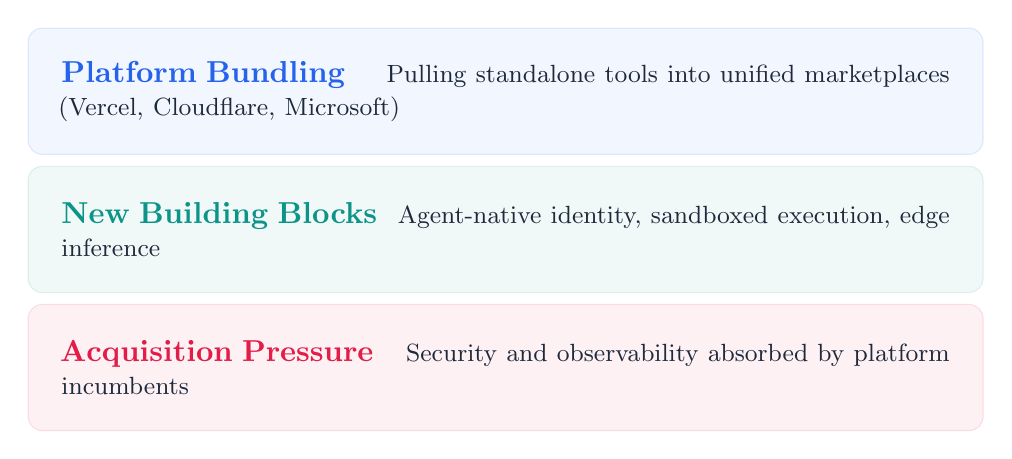
\begin{tikzpicture}[
  forcebox/.style={
    rectangle, rounded corners=5pt,
    minimum width=\textwidth, minimum height=16mm,
    inner sep=10pt, text width=\textwidth-24pt,
  },
]

\node[forcebox, fill=primary!6, draw=primary!15] (f1) at (0, 0) {
  {\fontsize{10.5}{13}\selectfont\bfseries\color{primary}Platform Bundling} \hfill
  {\fontsize{9.5}{12}\selectfont\color{textmain}Pulling standalone tools into unified marketplaces (Vercel, Cloudflare, Microsoft)}
};

\node[forcebox, fill=chartteal!6, draw=chartteal!15, below=4pt of f1] (f2) {
  {\fontsize{10.5}{13}\selectfont\bfseries\color{chartteal}New Building Blocks} \hfill
  {\fontsize{9.5}{12}\selectfont\color{textmain}Agent-native identity, sandboxed execution, edge inference}
};

\node[forcebox, fill=chartrose!6, draw=chartrose!15, below=4pt of f2] (f3) {
  {\fontsize{10.5}{13}\selectfont\bfseries\color{chartrose}Acquisition Pressure} \hfill
  {\fontsize{9.5}{12}\selectfont\color{textmain}Security and observability absorbed by platform incumbents}
};

\end{tikzpicture}

\vspace{14mm}

\insightbox{THE BOTTOM LINE}{Enterprise adoption data suggests genuine buyer intent---60\% plan to deploy agents within two years. But actual deployment lags far behind---only 17\% have done so. Whether the infrastructure stack proves durable or temporary depends on which of these numbers moves faster.}

\vspace{16mm}

\noindent\begin{tikzpicture}
  \fill[tableborder] (0,0) rectangle (\textwidth, 0.5pt);
\end{tikzpicture}

\vspace{6mm}

{\fontsize{9}{12}\selectfont\color{textsub}

\textbf{About this report.} This analysis covers 50+ companies that raised venture funding or were acquired for agent infrastructure functions between January 2024 and May 2026. Data sources include Crunchbase, PitchBook, SEC filings, company disclosures, and three enterprise surveys (McKinsey 2025, Gartner 2026, Deloitte 2026). The dataset is limited to disclosed funding and skews toward US-headquartered companies (approximately 82\% of captured capital).

\vspace{4mm}

\textbf{Author.} Vedang Ratan Vatsa $\cdot$ vedangvats@gmail.com

\vspace{4mm}

\textbf{Published.} May 2026

}

\end{document}
